\section{Результаты}

Описанная выше система управления персонажем

% Вот это тоже можно растянуть.
Описанное выше решение реализовано на языке Python с использованием библиотек pinocchio \cite{Carpentier}, \cite{Pinocchio} и cvxopt \cite{CVXOPT}

Тут какой-то текст не о чем.

% из полезного можно поговорить о том что видны изменения схожие с реальным движением человека.
% крч ты понял.

% NOTE: These values were selected experimentally
% \begin{figure}
%   \hfill
%   \begin{minipage}{0.327\textwidth}
%     \centering
%     \includegraphics[scale=0.091]{animation/1.png}
%   \end{minipage}
%   \begin{minipage}{0.327\textwidth}
%     \centering
%     \includegraphics[scale=0.091]{animation/2.png}
%   \end{minipage}
%   \begin{minipage}{0.327\textwidth}
%     \centering
%     \includegraphics[scale=0.091]{animation/3.png}
%   \end{minipage}
%   \vfill
%   \hfill
%   \begin{minipage}{0.327\textwidth}
%     \centering
%     \includegraphics[scale=0.091]{animation/4.png}
%   \end{minipage}
%   \begin{minipage}{0.327\textwidth}
%     \centering
%     \includegraphics[scale=0.091]{animation/5.png}
%   \end{minipage}
%   \begin{minipage}{0.327\textwidth}
%     \centering
%     \includegraphics[scale=0.091]{animation/6.png}
%   \end{minipage}
%   \vfill
%   \hfill
%   \begin{minipage}{0.327\textwidth}
%     \centering
%     \includegraphics[scale=0.091]{animation/7.png}
%   \end{minipage}
%   \begin{minipage}{0.327\textwidth}
%     \centering
%     \includegraphics[scale=0.091]{animation/8.png}
%   \end{minipage}
%   \begin{minipage}{0.327\textwidth}
%     \centering
%     \includegraphics[scale=0.091]{animation/9.png}
%   \end{minipage}
%   \vfill
%   \hfill
%   \begin{minipage}{0.327\textwidth}
%     \centering
%     \includegraphics[scale=0.091]{animation/10.png}
%   \end{minipage}
%   \begin{minipage}{0.327\textwidth}
%     \centering
%     \includegraphics[scale=0.091]{animation/11.png}
%   \end{minipage}
%   \begin{minipage}{0.327\textwidth}
%     \centering
%     \includegraphics[scale=0.091]{animation/12.png}
%   \end{minipage}
%   \vfill
%   \hfill
%   \begin{minipage}{0.327\textwidth}
%     \centering
%     \includegraphics[scale=0.091]{animation/13.png}
%   \end{minipage}
%   \begin{minipage}{0.327\textwidth}
%     \centering
%     \includegraphics[scale=0.091]{animation/14.png}
%   \end{minipage}
%   \begin{minipage}{0.327\textwidth}
%     \centering
%     \includegraphics[scale=0.091]{animation/15.png}
%   \end{minipage}
%   \vfill
%   \hfill
%   \begin{minipage}{0.327\textwidth}
%     \centering
%     \includegraphics[scale=0.091]{animation/16.png}
%   \end{minipage}
%   \begin{minipage}{0.327\textwidth}
%     \centering
%     \includegraphics[scale=0.091]{animation/17.png}
%   \end{minipage}
%   \begin{minipage}{0.327\textwidth}
%     \centering
%     \includegraphics[scale=0.091]{animation/18.png}
%   \end{minipage}
%   \caption{Анимация приседания}
% \end{figure}

% NOTE: These values were selected experimentally
% \begin{figure}
%   \hfill
%   \begin{minipage}{0.325\textwidth}
%     \centering
%     \includegraphics[scale=0.076]{balance/1.png}
%   \end{minipage}
%   \begin{minipage}{0.325\textwidth}
%     \centering
%     \includegraphics[scale=0.076]{balance/2.png}
%   \end{minipage}
%   \begin{minipage}{0.325\textwidth}
%     \centering
%     \includegraphics[scale=0.076]{balance/3.png}
%   \end{minipage}
%   \vfill
%   \hfill
%   \begin{minipage}{0.325\textwidth}
%     \centering
%     \includegraphics[scale=0.076]{balance/4.png}
%   \end{minipage}
%   \begin{minipage}{0.325\textwidth}
%     \centering
%     \includegraphics[scale=0.076]{balance/5.png}
%   \end{minipage}
%   \begin{minipage}{0.325\textwidth}
%     \centering
%     \includegraphics[scale=0.076]{balance/6.png}
%   \end{minipage}
%   \vfill
%   \hfill
%   \begin{minipage}{0.325\textwidth}
%     \centering
%     \includegraphics[scale=0.076]{balance/7.png}
%   \end{minipage}
%   \begin{minipage}{0.325\textwidth}
%     \centering
%     \includegraphics[scale=0.076]{balance/8.png}
%   \end{minipage}
%   \begin{minipage}{0.325\textwidth}
%     \centering
%     \includegraphics[scale=0.076]{balance/9.png}
%   \end{minipage}
%   \vfill
%   \hfill
%   \begin{minipage}{0.325\textwidth}
%     \centering
%     \includegraphics[scale=0.076]{balance/10.png}
%   \end{minipage}
%   \begin{minipage}{0.325\textwidth}
%     \centering
%     \includegraphics[scale=0.076]{balance/11.png}
%   \end{minipage}
%   \begin{minipage}{0.325\textwidth}
%     \centering
%     \includegraphics[scale=0.076]{balance/12.png}
%   \end{minipage}
%   \vfill
%   \hfill
%   \begin{minipage}{0.325\textwidth}
%     \centering
%     \includegraphics[scale=0.076]{balance/13.png}
%   \end{minipage}
%   \begin{minipage}{0.325\textwidth}
%     \centering
%     \includegraphics[scale=0.076]{balance/14.png}
%   \end{minipage}
%   \begin{minipage}{0.325\textwidth}
%     \centering
%     \includegraphics[scale=0.076]{balance/15.png}
%   \end{minipage}
%   \vfill
%   \hfill
%   \begin{minipage}{0.325\textwidth}
%     \centering
%     \includegraphics[scale=0.076]{balance/16.png}
%   \end{minipage}
%   \begin{minipage}{0.325\textwidth}
%     \centering
%     \includegraphics[scale=0.076]{balance/17.png}
%   \end{minipage}
%   \begin{minipage}{0.325\textwidth}
%     \centering
%     \includegraphics[scale=0.076]{balance/18.png}
%   \end{minipage}
%   \caption{Сбалансированная анимация приседания}
% \end{figure}
